
\section{CNN: tricks for visualization (Alfredo Canziani)}
% Authors: Pedro Manuel Herrero Vidal, Doruk Kilitcioglu
% Lecture date: 2/27/2019

We take the data simulated in the 04-spiral\_classification notebook (\href{https://github.com/Atcold/pytorch-Deep-Learning-Minicourse/blob/master/04-spiral\_classification.ipynb} {"Spiral Classification"}), 
consisting of 3,000 samples of dimension 2 (Fig. ~\ref{fig:NonLinearlySeparableParametricCurves2}). 
The data is generated from the following expression:

\[
X_c(t) = t
\begin{bmatrix}
    \sin{\frac{2\pi}{C} (2t+c+1) + \mathcal{N} (0, \sigma^2)} \\
    \cos{\frac{2\pi}{C} (2t+c+1) + \mathcal{N} (0, \sigma^2)}
\end{bmatrix}
\]
%\noindent
where $0 \leq t \leq 1$ and classes $c=1, ..., C$.


\begin{figure}[ht]
\centering
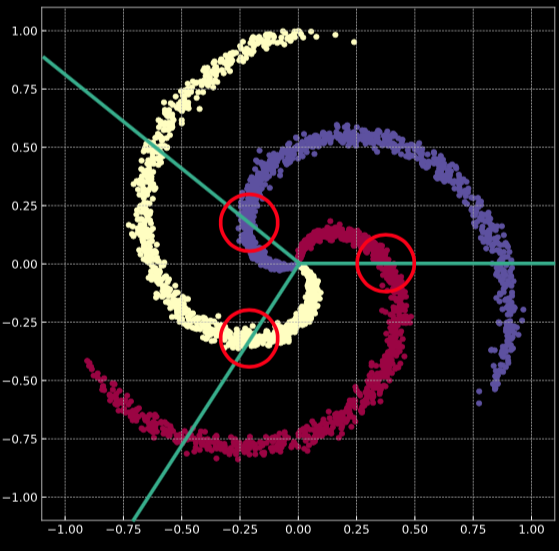
\includegraphics[width=0.5\textwidth]{lectures/04-a/images/NonLinearlySeparableParametricCurves.png}
\caption{3 non linearly separable curves consisting in 3,000 samples from $X \in {{\rm I\!R}}^2$.}
\label{fig:NonLinearlySeparableParametricCurves2}
\end{figure}

\noindent
To classify the data into the three categories, we are going to use a three layer net with: 
\begin{itemize}
\item[(1)] 2 input units (dimensionality of the data).
\item[(2)] A 100-units hidden layer (used to increase the space and extract features).
\item[(3)] Followed by a ReLU activation function that connects to a two-units layer (here is the trick for visualization!) 
\item[(4)] And then a linear transformation (with no non-linearity in between) to a 3-unit output layer with softmax activation function for classification 
(Fig. ~\ref{fig:ArchitectureForClassificationAndVisualizationInTheInputSpace}). 
Having a 2-unit layer (same as input layer) right before the output layer allows to visualize the transformations 
that the original space went throw to solve the classification task. 
The last linear transformation involves the multiplication of $A^{(3)}$ and $W^{(2)}$, 
where the different rows of $W^{(2)}$ are the 2D vectors that will point at the different classes in the 2D space. 
In this representation, the different classes are linearly separable.
\end{itemize}

\begin{figure}[!h]
\centering
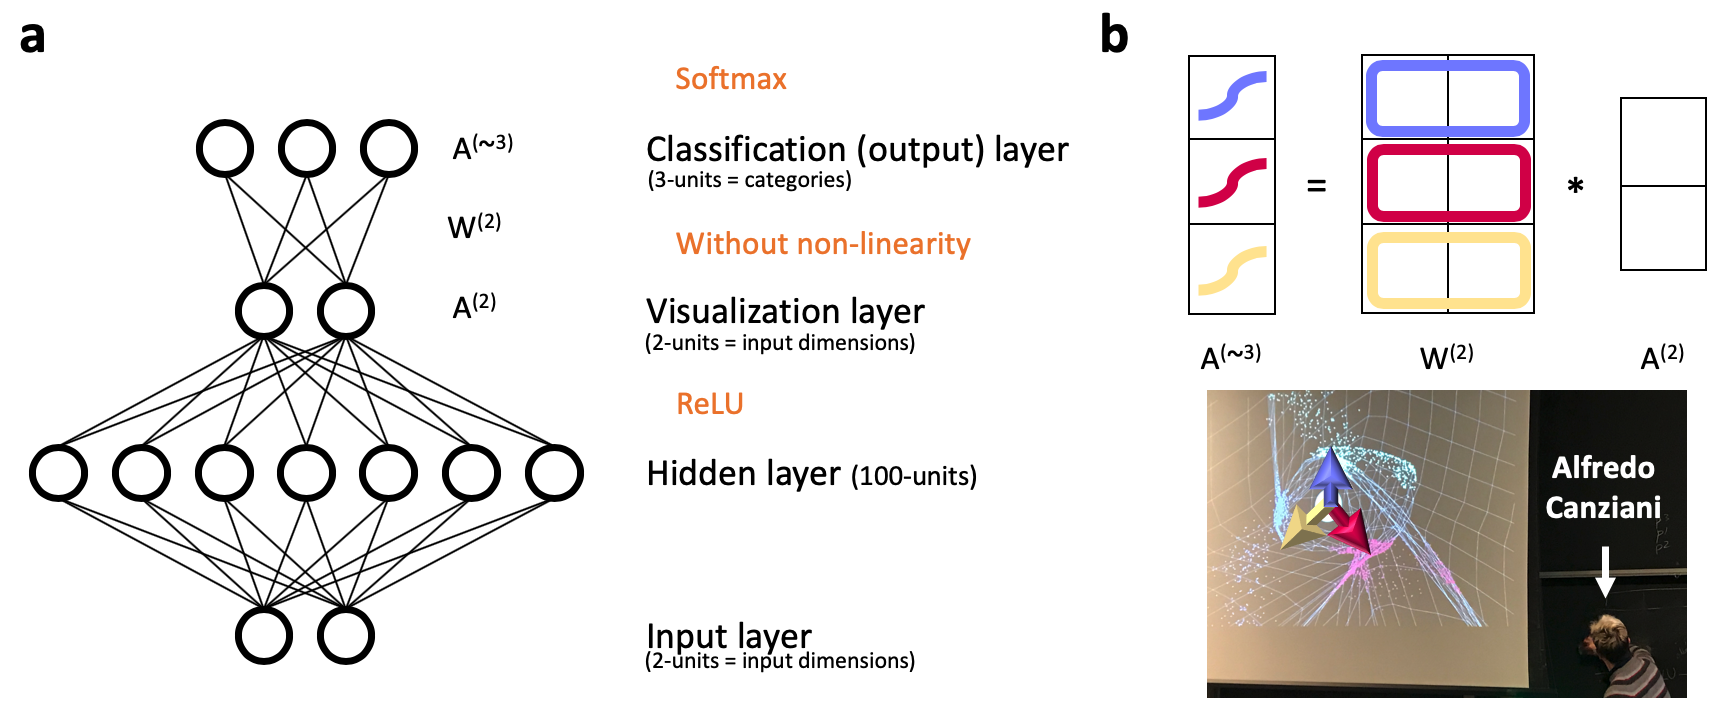
\includegraphics[width=170mm]{lectures/04-a/images/ArchitectureForClassificationAndVisualizationInTheInputSpace.png}
\caption{Neural network architecture for classification and visualization in the input space. (a) Architecture of the neural network, which takes 2D inputs and visualizes in the same dimensional space before classification. (b) Linear transformation that takes $A^{(2)}$ and returns $A^{(3)}$ via multiplication with $W^{(2)}$. Rectangular color boxes in $W^{(2)}$ represent the three 2D vectors that will define each class. Calculation of $A^{(3)}$ is followed by a softmax activation function for classification. In the bottom half of (b), the transformed data after and the population vectors (plot credit: Alfredo Canziani).}
\label{fig:ArchitectureForClassificationAndVisualizationInTheInputSpace}
\end{figure}

\noindent
We can linearly interpolate between the two data representations, before and 
after being feed into the network, in the 2D space by:

\[
(1-\alpha)(x^{(1)}) + \alpha \phi (x^{(i)}) ~~\text{ where } 0 \leq \alpha \leq 1
\]

\section{Convolution kernels}
\noindent
When applying a convolution transformation for a given layer of $N$ units and size of the kernel $K = 3$, 
it results in a layer of size $M = N-K+1$. However, this is only the case when the stride $S$ is 1 
and there is no skip (Fig. 3a). For a larger stride, or displacement of the kernel window in a given direction, 
the output dimensionality taking also padding $P$ into account is:

\[
 M = \frac{N + 2P - K}{S} + 1
\]

\noindent
This operation increases the subsampling rate, but helps speeding up the computation 
and may keep the relevant features for the task as well as assisting sample invariance (Fig. ~\ref{fig:ConvolutionATrou}). 
Another kind is the convolution 'a trou' ("with holes"). 
It applies a convolution kernel but skips a given number of inputs (Fig. ~\ref{fig:ConvolutionATrou}). 
Convolution 'a trou' results in an output with lower resolution than the input. 
However, when moving up the hierarchy units will pool inputs from several units after the 'a trou' convolution 
preserving the receptive field size of those neurons. In this case the output dimension is $M N(K-1)S_k +1$, being $S_k$ the skip size.

\begin{figure}[!h]
\centering
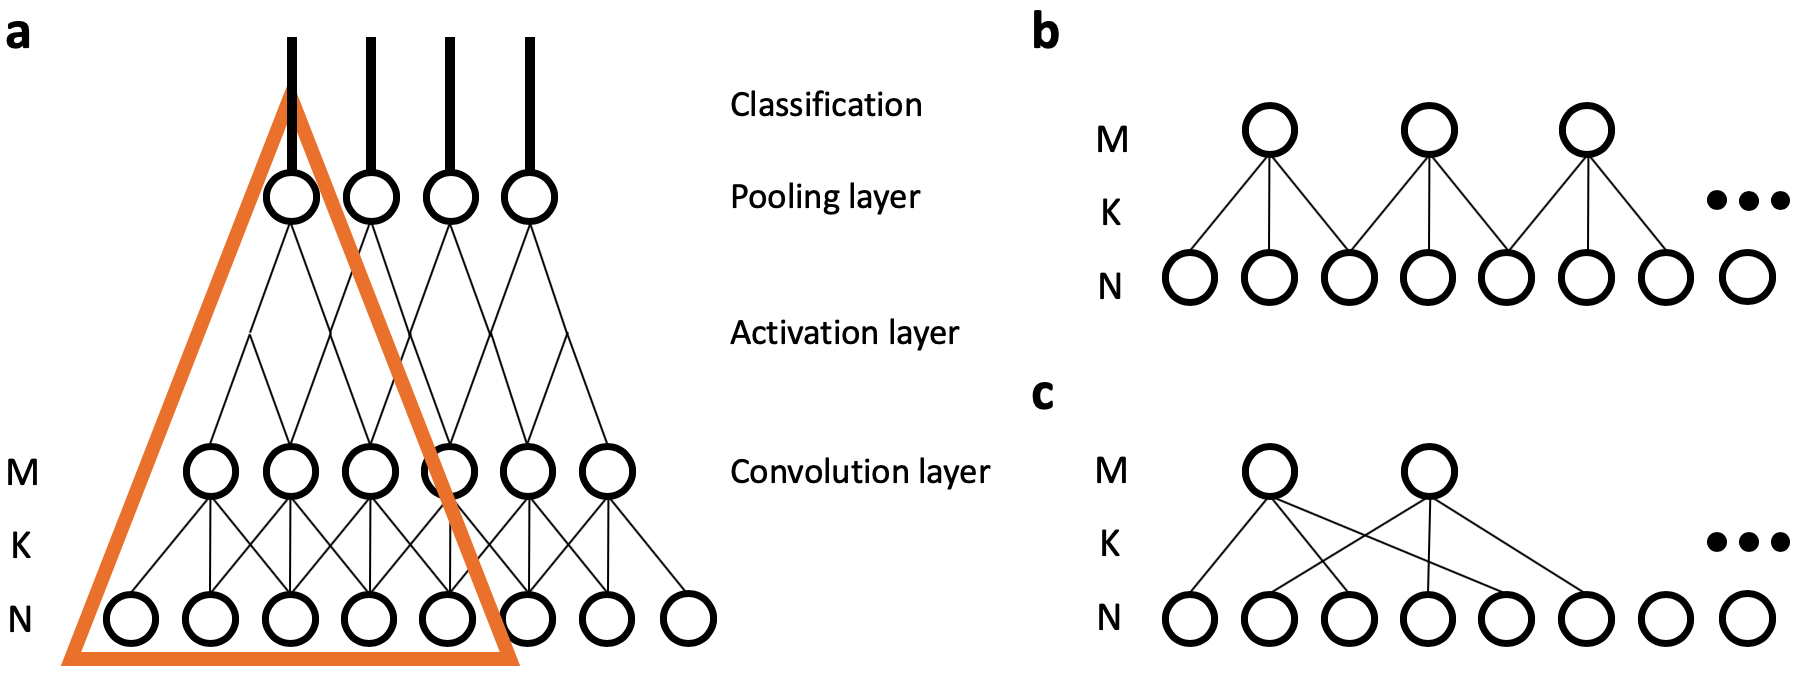
\includegraphics[width=170mm]{lectures/04-a/images/ConvolutionATrou.png}
\caption{Types of convolutions in a CNN module. (a) CNN module with input layer of size $N$ a kernel of size $K$ and output $M$, followed by and activation and pooling layers. Convolution with stride $2$ (b) and 'a trou' (c) diagrams.}
\label{fig:ConvolutionATrou}
\end{figure}

\vspace{4mm}
\noindent
In the context of images we want to be able to identify the desired categories independent of location and size. CNN exploit the locality, stationarity and compositionality of the input data using sparsness, parameter sharing and hierarchical structures, respectively. Therefore, we can use these networks to not only classify but also locate and segregate data. It is doubly beneficial because convolutions are computationally cheap; especially given that we can share parameters for a given convolution kernel (Fig. ~\ref{fig:ConvolutionATrou}, orange selection). Since it is common there is no need to recompute it. It also means that we can only get one output for a particular kernel. So, we can implement different kernels to the same input (increasing the depth of the representation), to extract different features. 

\subsection{Multiple character and face recognition}
\noindent
Properties of CNN allowed to train this networks to identify components regardless of size and location. If we apply those different kernels and give scores to each location for each of the classes and then determine that there was an object and which one it by the largest score. Higher scores are given to regions of the image with correct predictions and low to incorrect ones. This idea was implemented in the MNIST data set in the early 90s', for digit detection.

\vspace{4mm}
\noindent
Originally, face detection was originally implemented with customized features. In 1993 Vaillant et al. used CNN on large images for face detection (binary classification). It resulted in a large number of false positives, because face-like patterns are common in images. To prevent this from happening they added a second round of training with a training set that has no faces in them. Adding a hard negative mining step (train what 'no face' looks like enabled updated of the patches of the network that were incorrectly identifying faces. The CNN approach to face detection even at its early stages resulted in a significant improvement in the field. Furthermore, if we want to extract several features from the classification, for example, where are the faces and the orientation; it is better to train the same network to solve both tasks rather than training one per task. When training a network to solve all tasks at the same time, the CNN can generalize and use redundancy.


\section{Semantic segmentation}
\noindent
CNN can be use not only to identify but also segment images. This is important when dealing with biological images since we want to classify and know every pixel of the image. Manually labelled sets are required to train the net. Another application is self-driving vehicles. We may want to take images and label walk-able paths and obstacles. Before CNN, stereo-vision provided a solution where images can be segmented almost at real time, but with a limited depth range. Using the labelled examples from stereo-systems, we can train CNN to label and segment images using such features. It not only resulted in a comparable segmentation of the space but also overcame the depth restrains of stereo-vision. For the long range vision effect of neural networks, we can train it using scaled patches of the label set (just widen), making a depth impression for the network to learn. That way we can use the same kernel through the entire image. In 2010 another label set of 3,000 images was released. We can train CNN to identify the different categories to parse the scene and label it. Another strategy to produce segmented images is to generate an image of patches using super-pixel to define the boundaries, and then fill each of the patches with the label that is most 'voted' by the network in that section. 

\noindent
To identify categories regardless of location and size, a general recipe would be:
\begin{itemize}
\item[(1)] Use a CNN that takes as input the same imaged but scaled at different resolutions. 
\item[(2)] To prevent false alarms, we retrain the network using a set where the category of interest is not present. We can also incorporate sets with offset focus or non-centered representations of the object. 
\item[(3)] Apply non-maximum suppression. Decide the actual size of the object based on which scale of the image had the best score (or any other metric). 
\end{itemize}
